% =====================================================================
%  CT Dose AI — Technical and Clinical Report
%  Compile with:  pdflatex CT_Dose_AI_Report.tex   (run twice)
%  Requires: figs/*.png  (produced by docs/make_figs.py)
% =====================================================================
\documentclass[10pt,a4paper]{article}

% ---------- encoding & fonts ----------
\usepackage[T1]{fontenc}
\usepackage[utf8]{inputenc}
\usepackage{helvet}\renewcommand{\familydefault}{\sfdefault}
\usepackage{microtype}
\usepackage{amsmath,amssymb}

% ---------- layout ----------
\usepackage[a4paper,top=20mm,bottom=20mm,left=18mm,right=18mm]{geometry}
\usepackage{fancyhdr,titlesec,enumitem,parskip}
\usepackage{graphicx,booktabs,tabularx,array,colortbl,multirow}
\usepackage{xcolor,tcolorbox,tikz}
\usepackage[font=small,labelfont=bf,labelsep=period]{caption}
\usepackage[hidelinks]{hyperref}
\usetikzlibrary{arrows.meta,positioning,calc}
\tcbuselibrary{skins,breakable}

% ---------- palette ----------
\definecolor{ctblue}{HTML}{2A78D6}
\definecolor{ctbluedark}{HTML}{1A4F94}
\definecolor{ctaqua}{HTML}{1BAF7A}
\definecolor{ctorange}{HTML}{EB6834}
\definecolor{ctink}{HTML}{0B0B0B}
\definecolor{ctink2}{HTML}{52514E}
\definecolor{ctline}{HTML}{E2E2DE}
\definecolor{ctsurf}{HTML}{F7F7F5}
\definecolor{ctgreenbg}{HTML}{E8F6F0}

% ---------- headings ----------
\titleformat{\section}{\Large\bfseries\color{ctbluedark}}{\thesection\ \textperiodcentered\ }{0pt}{}[{\color{ctblue}\titlerule[1.4pt]}]
\titleformat{\subsection}{\large\bfseries\color{ctink}}{\thesubsection}{0.6em}{}
\titleformat{\subsubsection}{\normalsize\bfseries\color{ctink2}}{}{0pt}{}
\titlespacing*{\section}{0pt}{16pt}{8pt}
\titlespacing*{\subsection}{0pt}{12pt}{4pt}
\setlist[itemize]{leftmargin=14pt,itemsep=2pt,topsep=3pt}
\setlist[enumerate]{leftmargin=16pt,itemsep=2pt,topsep=3pt}

% ---------- header / footer ----------
\pagestyle{fancy}\fancyhf{}
\renewcommand{\headrulewidth}{0pt}
\renewcommand{\footrulewidth}{0.4pt}
\fancyfoot[L]{\footnotesize\color{ctink2}CT Dose AI \textperiodcentered\ project report}
\fancyfoot[R]{\footnotesize\color{ctink2}\thepage}

% ---------- shorthands ----------
\newcommand{\ctdi}{\ensuremath{\mathrm{CTDI}_{\mathrm{vol}}}}
\newcommand{\mgy}{mGy}
\newcommand{\mgycm}{mGy$\cdot$cm}

% ---------- boxes ----------
\newtcolorbox{callout}[1][]{enhanced,breakable,colback=ctsurf,colframe=ctblue,
  boxrule=0pt,leftrule=2.5pt,arc=2pt,left=8pt,right=8pt,top=6pt,bottom=6pt,#1}
\newtcolorbox{warnbox}[1][]{enhanced,breakable,colback=ctsurf,colframe=ctorange,
  boxrule=0pt,leftrule=2.5pt,arc=2pt,left=8pt,right=8pt,top=6pt,bottom=6pt,#1}
\newtcolorbox{safebox}[1][]{enhanced,breakable,colback=ctgreenbg,colframe=ctaqua,
  boxrule=0pt,leftrule=2.5pt,arc=2pt,left=8pt,right=8pt,top=6pt,bottom=6pt,#1}
\newtcolorbox{eqbox}{enhanced,colback=ctsurf,colframe=ctline,boxrule=0.5pt,arc=3pt,
  left=10pt,right=10pt,top=7pt,bottom=7pt}
% KPI tile
\newcommand{\kpi}[2]{%
  \begin{tcolorbox}[width=0.235\linewidth,colback=white,colframe=ctline,boxrule=0.6pt,arc=3pt,
      left=7pt,right=7pt,top=6pt,bottom=6pt,valign=top,nobeforeafter]
    {\fontsize{19}{21}\selectfont\bfseries\color{ctbluedark}#1}\\[3pt]
    {\footnotesize\color{ctink2}#2}
  \end{tcolorbox}}

\newcolumntype{R}{>{\raggedleft\arraybackslash}X}
\newcolumntype{L}{>{\raggedright\arraybackslash}X}
\renewcommand{\arraystretch}{1.25}
\newcommand{\hdr}{\rowcolor{ctsurf}}

\begin{document}
\thispagestyle{empty}

% =====================================================================
%  COVER
% =====================================================================
\vspace*{12mm}
{\footnotesize\bfseries\color{ctblue}\MakeUppercase{CT dose optimisation \ \textperiodcentered\ \ Project report}}

\vspace{4mm}
{\fontsize{30}{34}\selectfont\bfseries CT Dose AI}

\vspace{3mm}
{\large\color{ctink2} Predicting \ctdi{} and DLP for coronary CT angiography, and learning the lowest
radiation dose that still gives a diagnostic image.\par}

\vspace{7mm}
\noindent
\kpi{0.9\%}{\ctdi{} prediction error (cross-validated)}\hfill
\kpi{8.2\%}{DLP prediction error (cross-validated)}\hfill
\kpi{$\approx$40\%}{dose saving at 100~kV at equal estimated iodine CNR}\hfill
\kpi{50}{exams used to build and validate the model}

\vspace{8mm}
\noindent\textbf{What this document covers.} Sections~1--2 state the clinical problem and audit the data.
Section~3 describes the algorithm: the physics-informed prediction core, the recommendation engine, and the two
learning loops (Bayesian optimisation on a phantom, and a safe contextual bandit in clinical routine).
Section~4 shows the delivered application, Section~5 the measured results, Section~6 the open questions for the
data provider, and Section~7 limitations and next steps. Appendix~A holds the mathematics, Appendix~B the code map.

\vspace{3mm}
\begin{warnbox}
\textbf{\footnotesize\color{ctink2}\MakeUppercase{Status}}\\[2pt]
Research prototype and decision-support tool. It is \textbf{not} a medical device and has not been clinically
validated. Every protocol change must be reviewed by a medical physicist and the responsible radiologist before
use on patients.
\end{warnbox}

\vspace{4mm}
{\footnotesize\color{ctink2}
\textbf{\color{ctink}Contents.}
\textbf{1} The problem \quad
\textbf{2} The data and what it revealed \quad
\textbf{3} The algorithm (3.1 physics core, 3.2 model competition, 3.3 uncertainty,
3.4 recommendation engine, 3.5 phantom Bayesian optimisation, 3.6 safe contextual bandit) \quad
\textbf{4} The delivered solution \quad
\textbf{5} Results \quad
\textbf{6} Questions for the data provider \quad
\textbf{7} Limitations, safety, roadmap \quad
\textbf{A} Mathematical appendix \quad
\textbf{B} Code map \quad
\textbf{C} References\par}

\vfill
{\footnotesize\color{ctink2}\rule{\linewidth}{0.4pt}\\[3pt]
\textbf{\color{ctink}Author:} Thodoris Fragos \quad\textperiodcentered\quad
\textbf{\color{ctink}Data:} 50 coronary CT angiography exams (CARDIAC CT, provided by a clinical colleague)
\quad\textperiodcentered\quad \textbf{\color{ctink}Date:} 23 September 2026\\[2pt]
\textbf{\color{ctink}Repository:} \url{https://github.com/Thodoris1657/CT-Dose-AI-Algorithm}
\quad\textperiodcentered\quad
\textbf{\color{ctink}Stack:} Python, scikit-learn, SciPy, Streamlit, Plotly\par}

\clearpage

% =====================================================================
\section{The problem}

\subsection{The clinical request}
The project started from a request by a clinical colleague, who supplied the first batch of data:

\begin{callout}
\textit{``We want the AI programme (an app or a website, whichever you think) to take BMI, kVp, mAs and scan
length, and predict CTDI and DLP. First for this specific examination. Then we want to try other examinations too,
and to see whether --- and how --- it can find CTDI and DLP and suggest what I should change in kVp, mAs or scan
length in order to reduce CTDI and DLP. We consider BMI fixed, because it depends on the patient's height and
weight.''}
\end{callout}

That request contains two very different problems, and separating them is the key design decision of the project:

\begin{enumerate}
\item \textbf{A prediction problem.} Given the patient and the planned protocol, what dose will the scanner
deliver? This is a supervised-learning problem with a strong physical structure.
\item \textbf{A decision problem.} Which settings should change to lower the dose? A dose-only answer is trivial
and dangerous: the dose is minimised by scanning with almost no radiation, which produces useless images. The real
question is constrained --- \textit{the lowest dose that still yields a diagnostic image}. That constraint depends
on image quality, which is not present in the supplied data at all.
\end{enumerate}

\subsection{Why it matters}
Coronary CT angiography is one of the highest-dose routine CT examinations, and it is performed on patients who are
often young enough for stochastic risk to matter. National and European reference levels for CCTA are of the order
of 170--400~\mgycm{} for prospectively triggered protocols and 870--1060~\mgycm{} for retrospectively gated ones
[1,2]. The 50 supplied exams have a median DLP of about 1080~\mgycm, with a maximum of 2393~\mgycm.

\begin{figure}[h]
\centering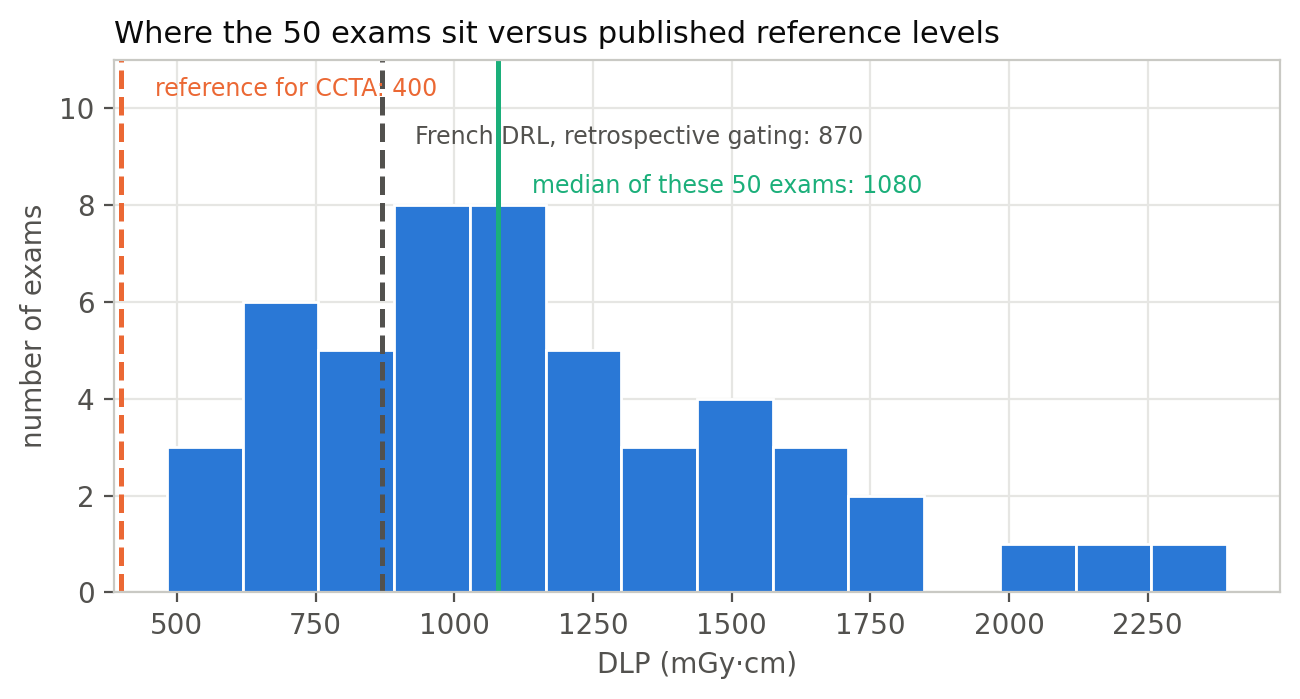
\includegraphics[width=0.82\linewidth]{figs/f4_drl.png}
\caption{DLP of the 50 supplied exams. The dose level is consistent with retrospectively gated acquisition at
120~kV. Almost every exam sits above the 400~\mgycm{} reference proposed for CCTA, which is where the opportunity
lies: there is real headroom to reduce dose, provided image quality is protected.}
\end{figure}

\subsection{What makes this hard}
\begin{itemize}
\item \textbf{Small data.} 50 exams, of which 48 are unique. Any model with many free parameters will memorise
noise. Validation has to be honest, or the project will produce an impressive-looking number and a useless tool.
\item \textbf{Narrow input range.} The data contains only 120~kV (46 exams) and 140~kV (4 exams). The most
effective dose-reduction lever --- dropping to 100~kV or 80~kV --- lies \textit{outside} the observed data. A purely
statistical model cannot extrapolate there; a physics-based one can, with a stated assumption.
\item \textbf{No image-quality signal.} Nothing in the data says whether an image was diagnostic. A recommendation
engine built on dose alone would simply recommend ``less''.
\item \textbf{BMI is fixed.} The one variable most correlated with dose is the one that cannot be changed. All the
levers are protocol parameters.
\end{itemize}

% =====================================================================
\section{The data and what it revealed}

The source file is a spreadsheet printed to PDF (\texttt{CARDIAC CT KARANISA.pdf}), with the columns split across
three blocks and six pages. The application parses it directly, so the same PDF can be re-imported at any time;
CSV and Excel are also supported.

\begin{table}[h]\footnotesize
\begin{tabularx}{\linewidth}{@{}l l r r L@{}}
\toprule
\hdr \textbf{Field} & \textbf{Role} & \textbf{Median} & \textbf{Range} & \textbf{Comment}\\
\midrule
Examination & grouping & \multicolumn{2}{c}{CCTA, all 50} & one model per exam type\\
BMI (kg/m\textsuperscript{2}) & input, fixed & 27.2 & 18.3--58.8 & patient property\\
kVp & input, tunable & 120 & 120 ($n{=}46$), 140 ($n{=}4$) & only two levels present\\
mAs & input, tunable & 756 & 375--1345 & set by tube-current modulation\\
Scan size (cm) & input, tunable & 29.8 & 22.4--44.2 & see the anomaly below\\
\ctdi{} (\mgy) & target & 47.5 & 21.1--105 & scanner console value\\
DLP (\mgycm) & target & 1080 & 482--2393 & scanner console value\\
\bottomrule
\end{tabularx}
\end{table}

\subsection{The automated data audit}
Before any model is fitted, the pipeline audits the data (\texttt{ctdose/data.py}). Four findings came out, and all
four are clinically informative.

\subsubsection{Finding 1 --- \ctdi{} is a deterministic function of mAs and kV}
\ctdi/mAs is essentially constant: 0.0605~\mgy/mAs at 120~kV and 0.0894~\mgy/mAs at 140~kV. This is not a
statistical correlation, it is the scanner's dose output per unit of tube charge. The ratio between the two kV
levels, 1.478, implies an exponent of 2.53 in $(\mathrm{kV}/120)^n$, squarely inside the physically expected
2.5--3.0 range. This single observation determines the entire modelling strategy.

\begin{figure}[h]
\centering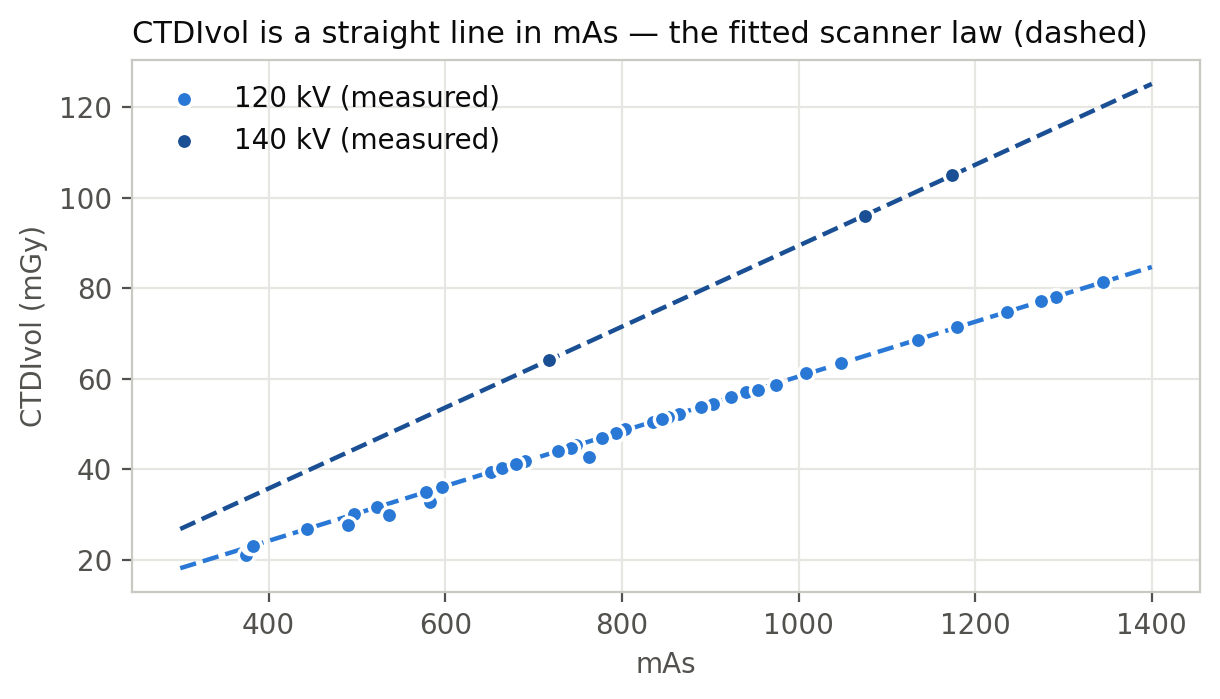
\includegraphics[width=0.78\linewidth]{figs/f1_physics.png}
\caption{Measured \ctdi{} against mAs, separated by tube voltage. The dashed lines are the fitted law, not a
regression through a cloud of points. The five points visibly below the 120~kV line are Finding~3.}
\end{figure}

\subsubsection{Finding 2 --- the ``SCAN SIZE CM'' field does not behave like the irradiated length}
DLP is, by definition, \ctdi{} multiplied by the irradiated length. Dividing the two gives an implied length of
$23.2 \pm 2.2$~cm. That implied length has \textit{no} positive correlation with the supplied scan-size field
($r = -0.23$), while the field itself correlates strongly with BMI ($r = +0.89$). The field therefore behaves like
a patient dimension or a field of view, not like $z$-coverage. This matters: it is the single largest source of
error in the DLP model.

\subsubsection{Finding 3 --- five exams have a different dose output per mAs}
Rows 2, 9, 22, 41 and 45 deliver about 7\% less \ctdi{} per mAs than the other 120~kV exams, and they cluster
tightly, which points to a systematic cause --- a different collimation, pitch or scan mode --- rather than noise.
Nothing in the four supplied inputs identifies them, so they set a floor on achievable accuracy.

\subsubsection{Finding 4 --- two pairs of duplicate rows}
Rows 28/43 and 29/42 are identical in every field. The pipeline keeps duplicates inside the same cross-validation
fold, so they cannot leak from training into testing and flatter the reported accuracy.

% =====================================================================
\clearpage
\section{The algorithm}

The system has one physics core and three layers built on it. The prediction layer answers \textit{what dose will
this protocol give?}; the recommendation layer answers \textit{what should I change?}; and two learning loops close
the gap the data cannot fill --- \textit{how low can we actually go?}

\begin{figure}[h]\centering
% Architecture diagram — shared by the report and the slides.
% Requires: tikz (arrows.meta, positioning), the ct* colours and \ctdi.
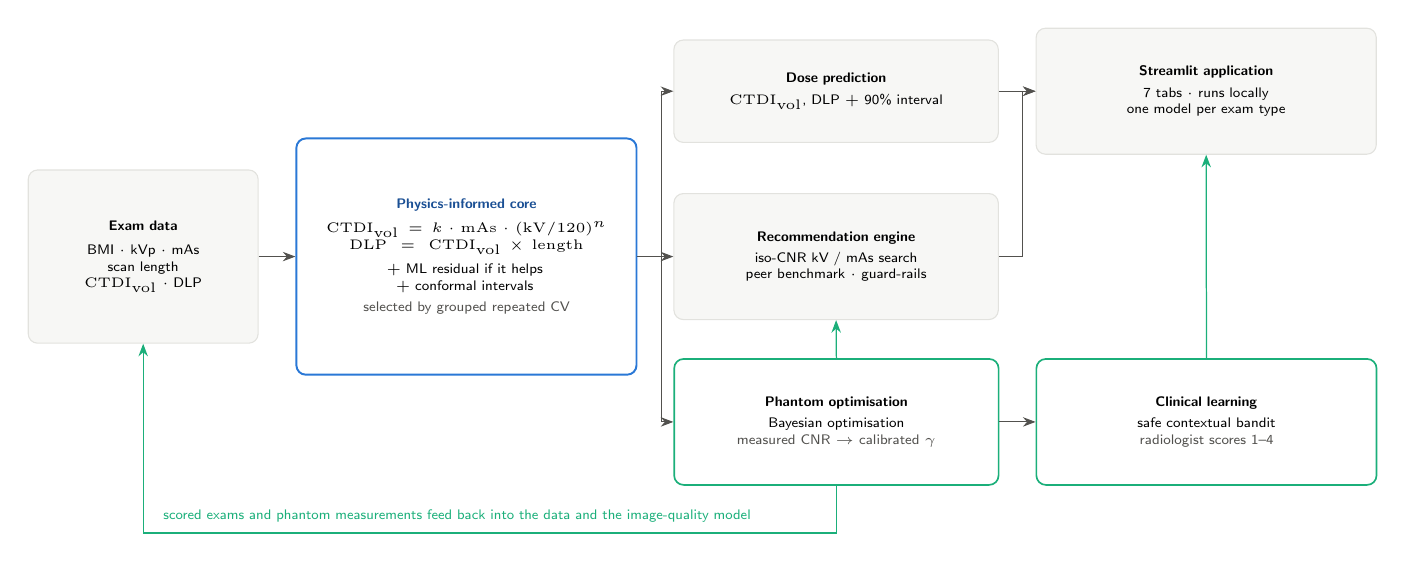
\begin{tikzpicture}[x=1mm,y=1mm,font=\sffamily\tiny,
  base/.style={rectangle,rounded corners=1.2mm,align=center,inner sep=1.6mm,anchor=west},
  box/.style={base,draw=ctline,fill=ctsurf},
  core/.style={base,draw=ctblue,line width=0.7pt,fill=white},
  loop/.style={base,draw=ctaqua,line width=0.6pt,fill=white},
  ar/.style={-{Stealth[length=1.6mm]},draw=ctink2,line width=0.35pt},
  arg/.style={-{Stealth[length=1.6mm]},draw=ctaqua,line width=0.45pt}]

\node[box,text width=26mm,minimum height=22mm] (data) at (0,0)
  {\textbf{Exam data}\\[1mm] BMI $\cdot$ kVp $\cdot$ mAs\\ scan length\\ \ctdi{} $\cdot$ DLP};

\node[core,text width=40mm,minimum height=30mm] (core) at (34,0)
  {\textbf{\textcolor{ctbluedark}{Physics-informed core}}\\[1mm]
   $\ctdi = k\cdot\mathrm{mAs}\cdot(\mathrm{kV}/120)^{n}$\\
   $\mathrm{DLP} = \ctdi \times \mathrm{length}$\\[1mm]
   $+$ ML residual if it helps\\ $+$ conformal intervals\\[0.6mm]
   {\color{ctink2}selected by grouped repeated CV}};

\node[box,text width=38mm,minimum height=13mm] (pred) at (82,21)
  {\textbf{Dose prediction}\\[0.6mm] \ctdi, DLP $+$ 90\% interval};

\node[box,text width=38mm,minimum height=16mm] (rec) at (82,0)
  {\textbf{Recommendation engine}\\[0.6mm] iso-CNR kV / mAs search\\ peer benchmark $\cdot$ guard-rails};

\node[loop,text width=38mm,minimum height=16mm] (bo) at (82,-21)
  {\textbf{Phantom optimisation}\\[0.6mm] Bayesian optimisation\\
   {\color{ctink2}measured CNR $\rightarrow$ calibrated $\gamma$}};

\node[box,text width=40mm,minimum height=16mm] (app) at (128,21)
  {\textbf{Streamlit application}\\[0.6mm] 7 tabs $\cdot$ runs locally\\ one model per exam type};

\node[loop,text width=40mm,minimum height=16mm] (band) at (128,-21)
  {\textbf{Clinical learning}\\[0.6mm] safe contextual bandit\\
   {\color{ctink2}radiologist scores 1--4}};

\draw[ar] (data.east) -- (core.west);
\draw[ar] (core.east) -- ++(3,0) |- (pred.west);
\draw[ar] (core.east) -- (rec.west);
\draw[ar] (core.east) -- ++(3,0) |- (bo.west);
\draw[ar] (pred.east) -- (app.west);
\draw[ar] (rec.east) -- ++(3,0) |- (app.west);
\draw[ar] (bo.east) -- (band.west);
\draw[arg] (bo.north) -- (rec.south);
\draw[arg] (band.north) -- (app.south);
\draw[arg] (bo.south) -- ++(0,-6) -| (data.south);
\node[font=\sffamily\tiny,text=ctaqua,anchor=west] at (16,-33)
  {scored exams and phantom measurements feed back into the data and the image-quality model};
\end{tikzpicture}

\caption{System architecture. Blue = the dose model built from the supplied data; green = the two loops that
acquire the image-quality information the data does not contain.}
\end{figure}

\subsection{Physics-informed prediction core}
All models work in log space, because dose quantities are positive and their drivers multiply. The physical law for
a given scanner is:

\begin{eqbox}
$\displaystyle \ctdi = k \cdot \mathrm{mAs} \cdot (\mathrm{kVp}/120)^{n}
\;\Longrightarrow\; \log \ctdi = \log k + \mathbf{1}\cdot\log \mathrm{mAs} + n\log(\mathrm{kVp}/120)$\\[4pt]
$\displaystyle \mathrm{DLP} = \ctdi \times L_{\text{irradiated}}
\;\Longrightarrow\; \log \mathrm{DLP} = \log \ctdi + \log L$
\end{eqbox}

Two modelling choices follow, and both are deliberate:
\begin{itemize}
\item \textbf{The mAs exponent is fixed at 1}, not fitted. Dose is linear in tube charge by definition. Fixing it
means the model extrapolates safely to mAs values never seen in training, and removes one parameter from a 48-row
dataset.
\item \textbf{The fit is robust (Huber loss)}, so the five deviant exams from Finding~3 do not drag the fitted
constant away from the behaviour of the other 45.
\end{itemize}
Fitted values for this scanner: $k = 0.0605$~\mgy/mAs and $n = 2.53$. The DLP model adds a fitted effective length,
which absorbs the fact that the true $z$-coverage is not recorded.

\subsection{Model competition and validation}
The physics law was not assumed to be best --- it had to win a competition against eight alternatives, including
black-box models, under an identical protocol:
\begin{itemize}
\item \textbf{Candidates:} physics law; physics $+$ BMI; physics $+$ length; physics $+$ Gaussian-process residual;
physics $+$ neural-network residual; physics $+$ gradient-boosting residual; log--log ridge regression with
interactions; gradient boosting with monotonicity constraints on mAs and kV; and a bagged ensemble of deep
multilayer perceptrons (the ``deep learning'' entry).
\item \textbf{Protocol:} repeated grouped 5-fold cross-validation, 10 repeats (50 fits per model). Duplicate rows
are forced into the same fold.
\item \textbf{Selection:} the 1-standard-error rule --- the simplest model whose error is within one standard error
of the best. This prevents a complex model winning on a fluctuation.
\end{itemize}

\begin{figure}[h]
\centering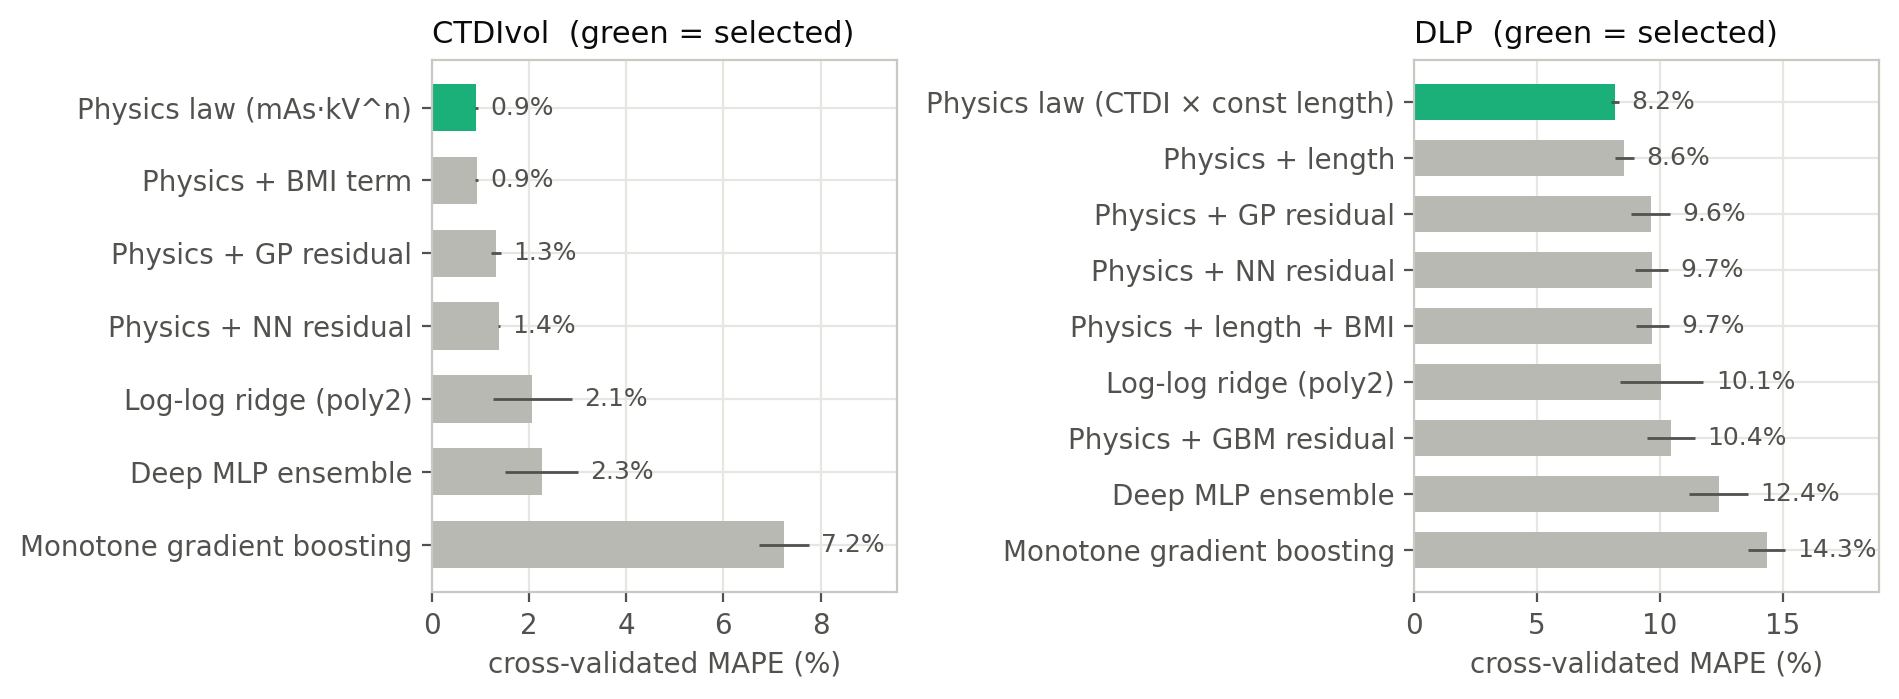
\includegraphics[width=\linewidth]{figs/f2_benchmark.png}
\caption{Cross-validated mean absolute percentage error, with the spread across repeats. For both targets the
physics-informed model wins outright. The deep ensemble is 2.5$\times$ worse on \ctdi{} and 1.5$\times$ worse on
DLP --- the expected outcome with 48 unique rows and a known functional form.}
\end{figure}

\begin{table}[h]\footnotesize
\begin{tabularx}{\linewidth}{@{}L r r r r@{}}
\toprule
\hdr \textbf{Model} & \textbf{\ctdi{} error} & \textbf{R\textsuperscript{2}} & \textbf{DLP error} & \textbf{R\textsuperscript{2}}\\
\midrule
\rowcolor{ctgreenbg}\textbf{Physics law (selected)} & \textbf{0.92\% $\pm$ 0.03} & \textbf{0.998} & \textbf{8.17\% $\pm$ 0.17} & \textbf{0.922}\\
Physics $+$ Gaussian-process residual & 1.32\% & 0.998 & 9.63\% & 0.854\\
Physics $+$ neural-network residual & 1.38\% & 0.998 & 9.66\% & 0.849\\
Log--log ridge with interactions & 2.07\% & 0.960 & 10.07\% & 0.734\\
Deep MLP ensemble & 2.26\% & 0.964 & 12.39\% & 0.586\\
Monotone gradient boosting & 7.25\% & 0.838 & 14.35\% & 0.695\\
\bottomrule
\end{tabularx}
\end{table}

\begin{figure}[h]
\centering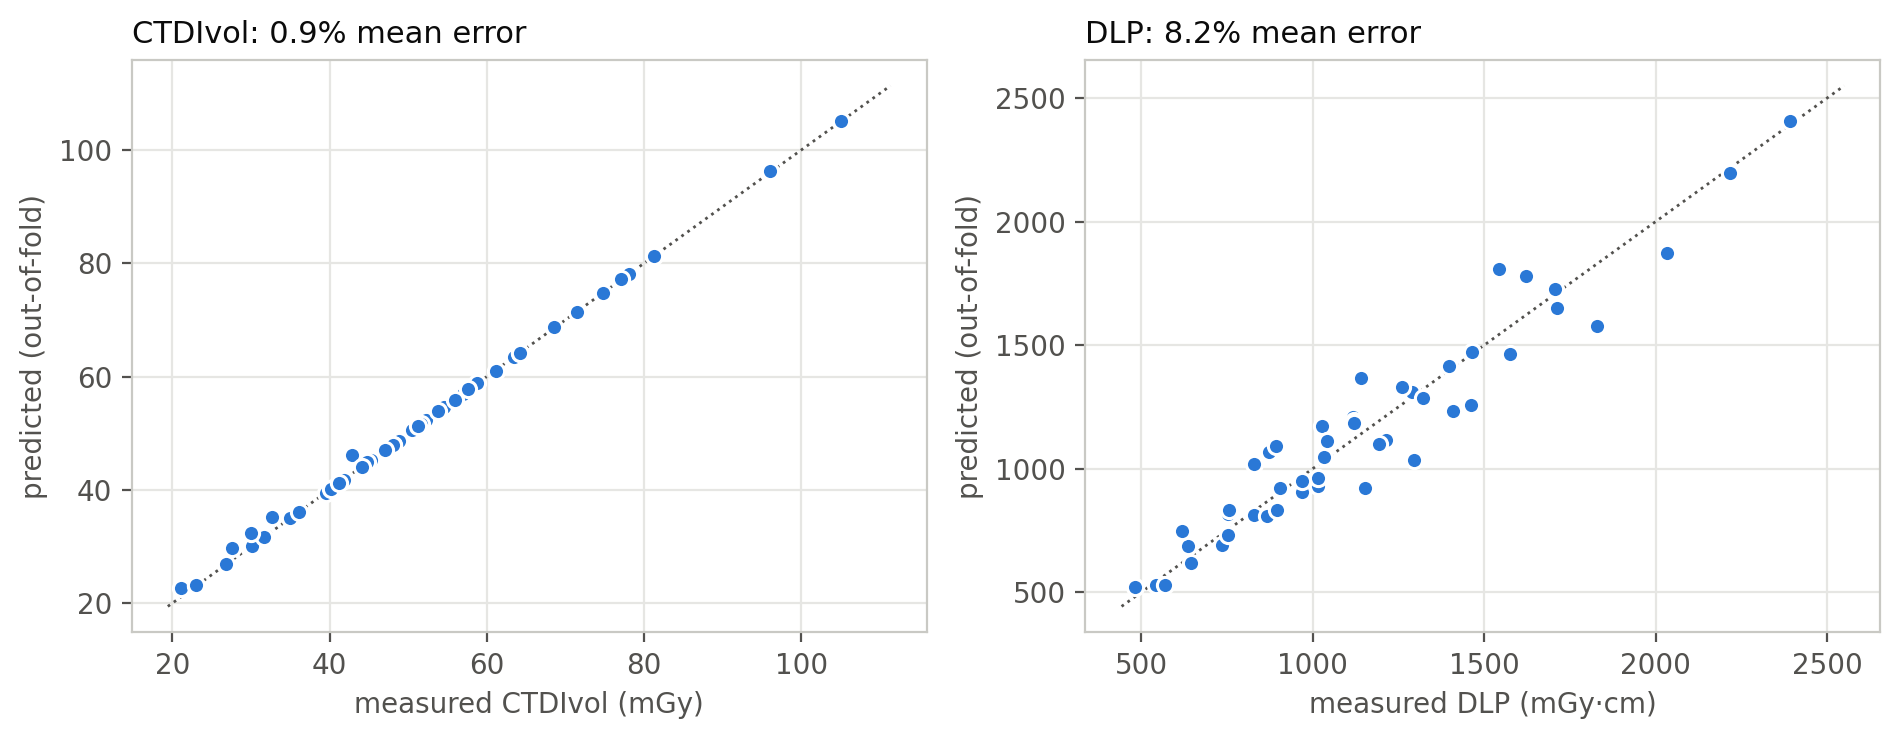
\includegraphics[width=\linewidth]{figs/f3_oof.png}
\caption{Out-of-fold predictions (every point predicted by a model that never saw it). \ctdi{} lies on the identity
line except for the five deviant exams; the DLP scatter reflects the unrecorded scan length.}
\end{figure}

\begin{safebox}
\textbf{\footnotesize\color{ctink2}\MakeUppercase{Why the simple model is the right answer, not a shortcut}}\\[2pt]
A deep network is the correct tool when the functional form is unknown and data is plentiful. Here the form is
known exactly and the data is scarce, so the network spends its capacity re-learning a straight line from 48 points
--- and does it worse. The value added by machine learning in this project is not in the function approximator; it
is in the validation protocol, the calibrated uncertainty, the constrained optimisation, and the two
active-learning loops. Should the dataset grow to thousands of exams with heart rate, pitch, gating mode and
reconstruction level, the same script re-runs the full competition and will select a flexible model automatically
if one then wins.
\end{safebox}

\clearpage
\subsection{Uncertainty and applicability domain}
A point prediction without an error bar invites misuse, so every prediction carries a \textbf{conformal prediction
interval} calibrated on out-of-fold residuals. Conformal intervals are distribution-free: they guarantee the stated
coverage under exchangeability, without assuming normal errors.

\begin{table}[h]\footnotesize
\begin{tabularx}{\linewidth}{@{}l l r L@{}}
\toprule
\hdr \textbf{Target} & \textbf{90\% interval (multiplicative)} & \textbf{Coverage} & \textbf{Interpretation}\\
\midrule
\ctdi{} & prediction $\times\,[0.927,\ 1.003]$ & 94\% & asymmetric: the lower tail is the 7\% deviant cluster\\
DLP & prediction $\times\,[0.820,\ 1.248]$ & 94\% & width reflects the unknown scan length\\
\bottomrule
\end{tabularx}
\end{table}

In addition, every prediction is checked against the \textbf{applicability domain}. Inputs outside the training
ranges are flagged, and any kV value not present in the data (80, 90, 100~kV) produces an explicit warning that the
estimate relies on the fitted physics kV-law rather than on observed exams. The tool states when it is
extrapolating instead of hiding it.

\subsection{Dose-reduction recommendation engine}
Dose alone is not a valid objective, so the engine optimises dose \textit{subject to an image-quality constraint}.
For the same patient, quantum noise falls with the square root of dose, while iodine contrast rises as the tube
voltage approaches the iodine K-edge:

\begin{eqbox}
$\displaystyle \sigma_{\text{noise}} \propto 1/\sqrt{\ctdi} \qquad
C_{\text{iodine}} \propto \mathrm{kVp}^{-\gamma},\quad \gamma \approx 1.2\text{--}1.5$\\[4pt]
$\displaystyle \mathrm{CNR_{rel}} = \left(\frac{\mathrm{kVp_{old}}}{\mathrm{kVp_{new}}}\right)^{\!\gamma}
\sqrt{\frac{D_{\mathrm{new}}}{D_{\mathrm{old}}}}
\qquad\text{hold } \mathrm{CNR} \ge \tau:\quad
D_{\mathrm{new}} \ge D_{\mathrm{old}}\,\tau^{2}
\left(\frac{\mathrm{kVp_{new}}}{\mathrm{kVp_{old}}}\right)^{\!2\gamma}$\\[3pt]
{\footnotesize\color{ctink2}($D$ denotes \ctdi{}; $\tau$ is the fraction of the current CNR to preserve.)}
\end{eqbox}

This is why lowering kV is the dominant lever in contrast-enhanced CT: at 100~kV the same iodine CNR needs about
40\% less dose than at 120~kV. The engine evaluates every available kV, computes the mAs that preserves the chosen
fraction of the current CNR, and ranks the results. Four guard-rails constrain the search:
\begin{itemize}
\item \textbf{Minimum kV by BMI} (default 80~kV below BMI 25, 100~kV for 25--30, 120~kV above 30), following
PROTECTION VI [1] --- this prevents photon starvation in large patients.
\item \textbf{Tube output limits}: options that would exceed the tube's maximum mAs are marked as unable to reach
the CNR target.
\item \textbf{Peer benchmark}: quantile regression of the local data gives the median and 25th-percentile dose
actually used for patients of the same BMI --- an ``achievable dose'' that needs no extrapolation at all.
\item \textbf{Scan length}: DLP is proportional to irradiated length, so the saving per centimetre is reported
separately, with the caveat from Finding~2 attached.
\end{itemize}

\begin{figure}[h]
\centering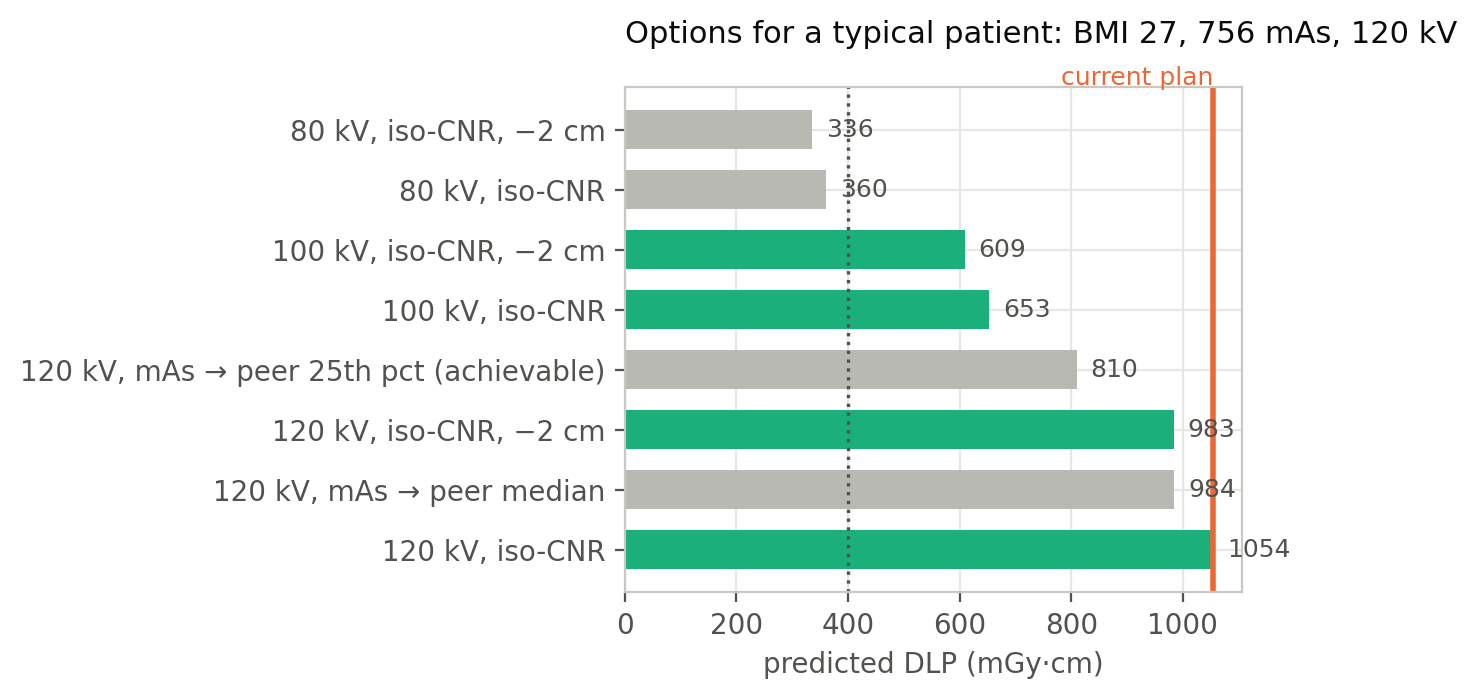
\includegraphics[width=0.85\linewidth]{figs/f5_options.png}
\caption{Ranked options for a median patient (BMI 27, 756~mAs, 120~kV; predicted 45.7~\mgy{} and 1056~\mgycm).
Green options satisfy every constraint. The recommendation is 100~kV / 735~mAs, which is $-39\%$ \ctdi{} and
$-42\%$ DLP with 2~cm less coverage, at the same estimated iodine CNR. The 80~kV options are greyed out because
the patient's BMI exceeds the 80~kV rule.}
\end{figure}

\clearpage
\subsection{Phantom Bayesian optimisation}
The CNR model above uses a literature exponent. The honest way to replace it with a measured one is a phantom
experiment --- but scanning a full grid of kV $\times$ mAs combinations wastes scanner time. Bayesian optimisation
solves exactly this: choose each next measurement so that it is maximally informative about the optimum.
\begin{itemize}
\item \textbf{Objective:} minimise \ctdi{} subject to measured CNR $\ge$ target. Dose is known analytically from
the fitted scanner law; CNR is the unknown, noisy, expensive function.
\item \textbf{Surrogate:} $\log \mathrm{CNR} = b_0 - \gamma\log(\mathrm{kV}/120) + \delta\log \ctdi$,
fitted as a Bayesian linear model with physics priors ($\gamma \approx 1.35 \pm 0.5$, $\delta \approx 0.5 \pm
0.15$), plus a Gaussian-process residual that captures what the formula misses, such as photon starvation at low
kV. The priors are what make the method useful after 2--3 scans instead of 30.
\item \textbf{Acquisition:} constrained expected improvement,
$a(x) = \max(0,\ d^{*} - d(x)) \cdot P(\mathrm{CNR}(x) \ge \text{target})$. Before any feasible point exists it
takes the lowest-dose setting that is more likely than not to pass.
\item \textbf{Output:} the next scan to perform, the recommended protocol, and a \textbf{calibrated $\gamma$} that
replaces the literature value in the recommendation engine.
\end{itemize}

\begin{figure}[h]
\centering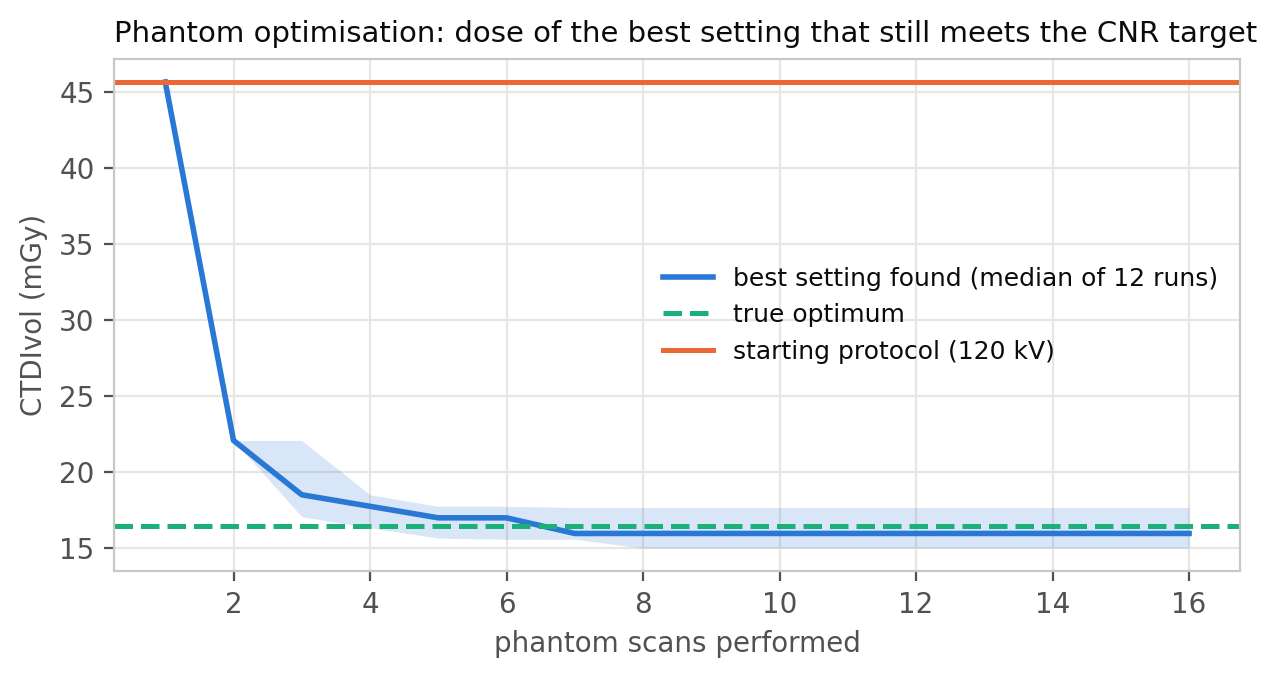
\includegraphics[width=0.8\linewidth]{figs/f6_bo.png}
\caption{Simulated campaigns on a synthetic phantom (12 runs, band $=$ 10th--90th percentile). The starting
protocol is the current clinical one. After about 7 scans the procedure sits at the true constrained optimum ---
roughly 65\% below the starting dose in this simulation. The curve can dip marginally below the true optimum
because a single noisy measurement may pass the target by chance, which is why the reported recommendation uses the
95\% posterior probability rather than the best single measurement.}
\end{figure}

\subsection{Safe contextual bandit in clinical routine}
A phantom is not a patient. The final loop learns from clinical practice itself, using the one signal that defines
success: whether the radiologist found the image diagnostic.
\begin{itemize}
\item \textbf{Context:} the patient's BMI. \textbf{Actions:} combinations of kV and image-quality level, converted
into concrete mAs through the scanner law. \textbf{Reward:} a 1--4 diagnostic-quality score, with $\ge 3$ counted as
acceptable.
\item \textbf{Model:} Bayesian logistic regression (Laplace approximation) of $P(\text{acceptable})$ on BMI,
$\log$ \ctdi{} and $\log$ kV, with physics-informed priors --- more dose helps, lower kV helps iodine contrast at
equal dose, a larger patient is harder. A single shared model means every exam informs every arm, which is far more
data-efficient than learning each protocol independently.
\item \textbf{Decision:} Thompson sampling. One plausible model is drawn from the posterior, and the lowest-dose
allowed action whose sampled $P(\text{acceptable})$ clears the target (default 0.97) is proposed. Exploration comes
from the posterior draw and shrinks automatically as evidence accumulates.
\end{itemize}

\begin{safebox}
\textbf{\footnotesize\color{ctink2}\MakeUppercase{Four safety rails, all active simultaneously}}
\begin{enumerate}
\item The BMI minimum-kV rule always applies.
\item The pessimistic (10th-percentile) posterior $P(\text{acceptable})$ of a proposal must exceed 0.85.
\item A proposal may be at most 15\% below the lowest dose already \textit{proven} acceptable for a similar BMI
($\pm 3$ BMI units), so the dose descends in small, evidenced steps rather than jumping.
\item A radiologist approves or overrides every single proposal, and the override is recorded.
\end{enumerate}
\end{safebox}

\begin{figure}[h]
\centering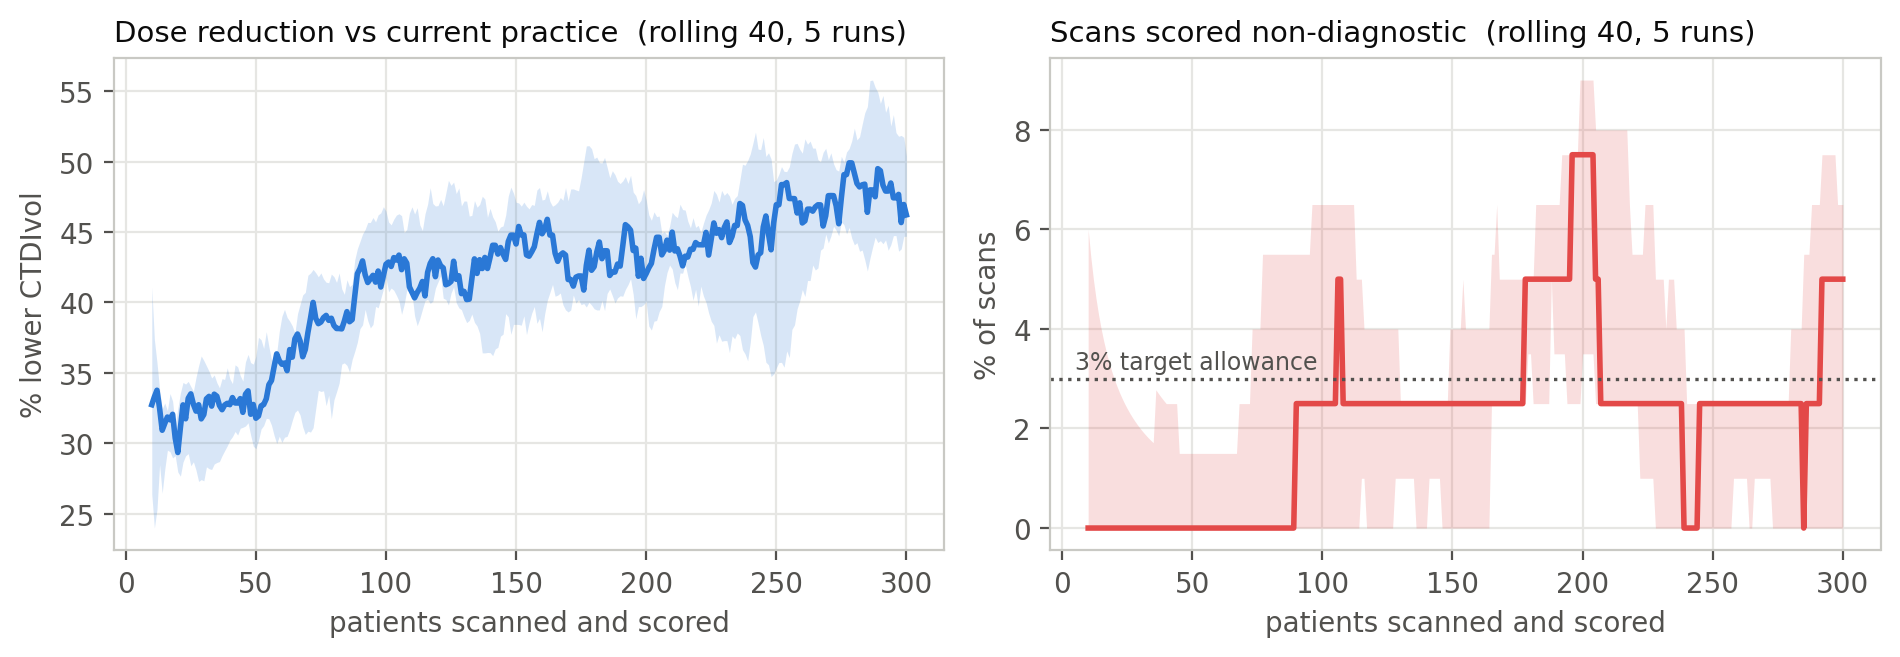
\includegraphics[width=\linewidth]{figs/f7_bandit.png}
\caption{Simulation with a synthetic reader whose acceptance depends on true iodine CNR (5 runs $\times$ 300
patients; line $=$ median, band $=$ 10th--90th percentile). Dose falls about 32\% immediately --- this comes from
the kV switch, which the physics prior already considers safe --- and reaches 45--50\% as evidence accumulates. The
non-diagnostic rate stays near the 3\% allowance implied by the 0.97 target, which is the parameter the department
sets.}
\end{figure}

% =====================================================================
\clearpage
\section{The delivered solution}
Everything above ships as a local Python application: \texttt{python app.py} opens it in a browser. Nothing leaves
the computer, which matters for patient data. Seven tabs cover the workflow.

\begin{figure}[h]\centering
\begin{minipage}[t]{0.49\linewidth}\centering
  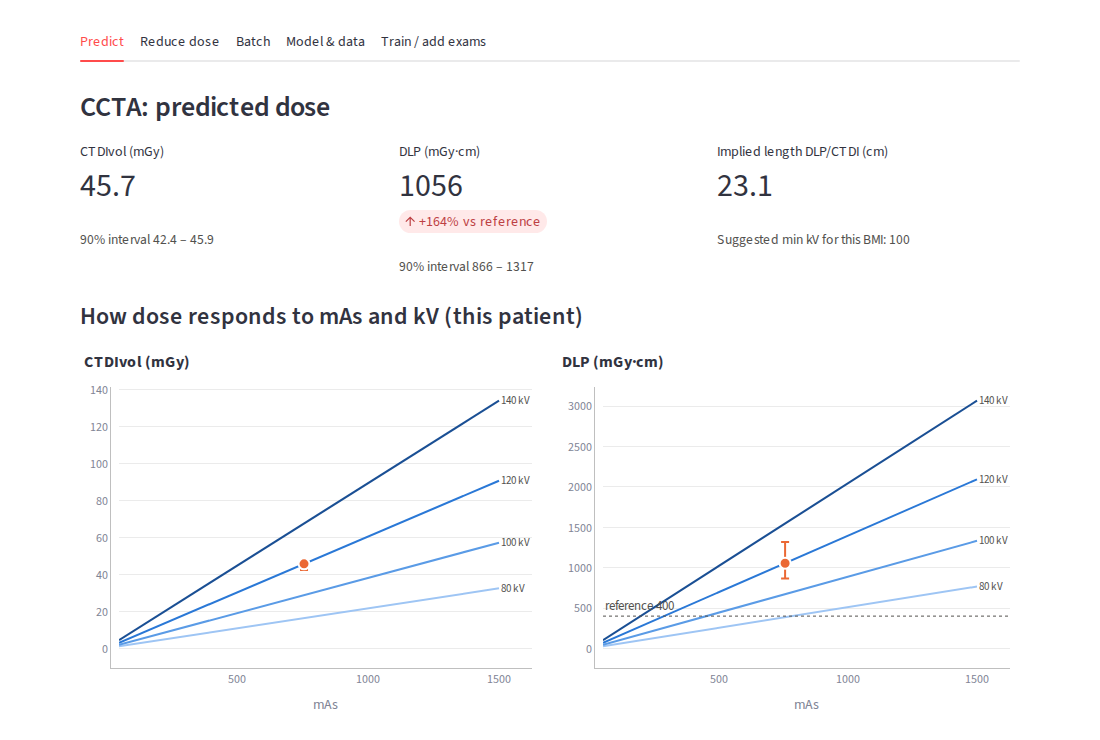
\includegraphics[width=\linewidth]{figs/app_predict.png}
  \captionof{figure}{\textbf{Predict} --- dose with 90\% intervals, comparison against the reference level, and the
  dose response to mAs at each kV for this patient.}
\end{minipage}\hfill
\begin{minipage}[t]{0.49\linewidth}\centering
  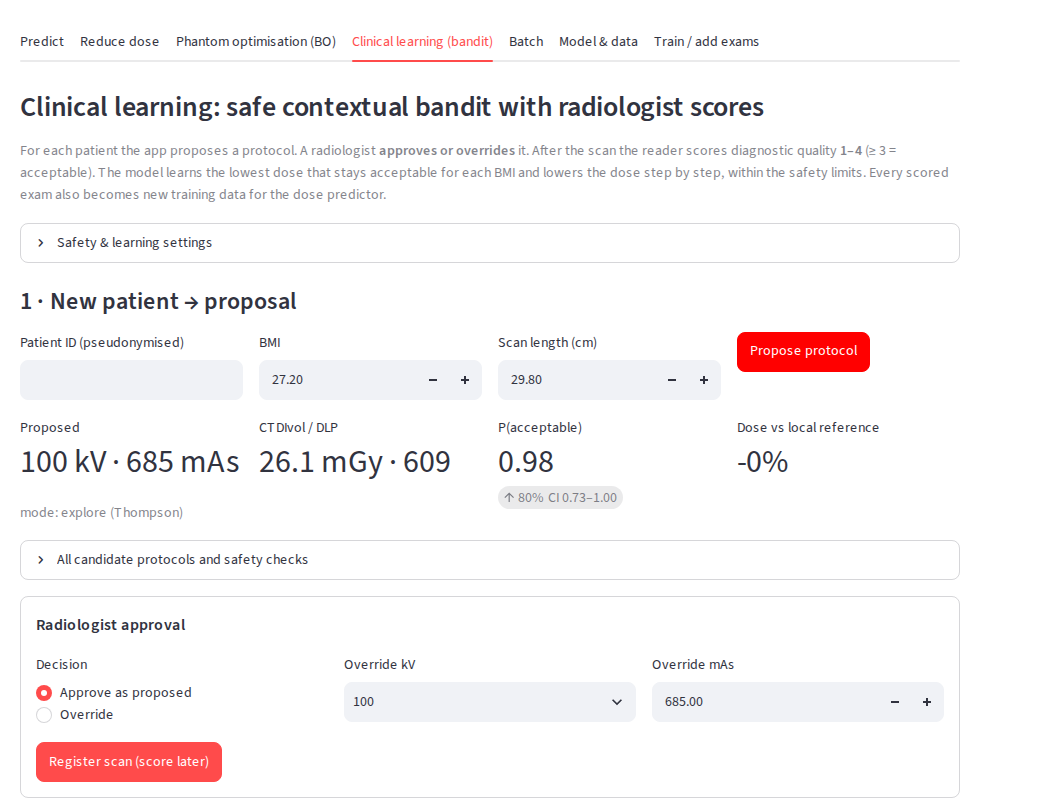
\includegraphics[width=\linewidth]{figs/app_bandit.png}
  \captionof{figure}{\textbf{Clinical learning} --- proposal, probability of acceptability with its credible
  interval, approval control, and the learned curves.}
\end{minipage}
\end{figure}

\begin{table}[h]\footnotesize
\begin{tabularx}{\linewidth}{@{}l L l@{}}
\toprule
\hdr \textbf{Tab} & \textbf{What it does} & \textbf{Who uses it}\\
\midrule
\textbf{Predict} & \ctdi{} and DLP with 90\% intervals, reference-level comparison, dose-response curves, out-of-domain warnings & radiographer, physicist\\
\textbf{Reduce dose} & Ranked protocol options at constant estimated CNR, peer benchmark, guard-rails, manual what-if panel & physicist, radiologist\\
\textbf{Phantom optimisation} & Proposes the next phantom scan, accepts the measured CNR, returns the optimal protocol and calibrated $\gamma$ & physicist\\
\textbf{Clinical learning} & Per-patient proposal $\rightarrow$ approval $\rightarrow$ 1--4 score $\rightarrow$ model update; dashboards and export & radiologist\\
\textbf{Batch} & Predicts a whole CSV/Excel/PDF file and reports errors when true doses are present & physicist, audit\\
\textbf{Model \& data} & Model card: cross-validation table, fitted law, out-of-fold plots, full data audit & reviewer, physicist\\
\textbf{Train / add exams} & Upload another exam type; it gets its own model and report automatically & anyone\\
\bottomrule
\end{tabularx}
\end{table}

\subsection{How the loops close}
The three components feed each other, which is what makes this a system rather than three scripts:
\begin{enumerate}
\item The phantom campaign produces a measured $\gamma$, which replaces the literature value in the recommendation
engine and in the bandit's action set.
\item Every clinically scored exam updates the acceptability model, and the ``Reduce dose'' tab then displays the
lowest dose proven acceptable for that BMI, drawn from local evidence rather than from physics assumptions.
\item Scored exams whose \ctdi{} and DLP were read from the console are appended to the training data, so the next
\texttt{python train.py} re-runs the whole model competition on a larger dataset. The dataset grows by itself
through routine use.
\end{enumerate}

\subsection{Engineering quality}
The test suite (13 automated tests) covers the data schema and duplicate grouping, recovery of a known physics law
from synthetic data, monotonicity of predictions in mAs and kV, interval consistency, optimiser constraint
compliance (including that an obese patient never receives a sub-120~kV proposal), surrogate recovery of a known
$\gamma$, convergence of the Bayesian optimisation to within 25\% of a known optimum, and the bandit's safety and
learning behaviour. Training writes a versioned model card and a markdown report for each exam type. The
application retrains itself automatically when the installed scikit-learn version differs from the one that
produced the stored models.

% =====================================================================
\section{Results}

\begin{table}[h]\footnotesize
\begin{tabularx}{\linewidth}{@{}L l L@{}}
\toprule
\hdr \textbf{Question} & \textbf{Answer} & \textbf{Evidence}\\
\midrule
Can \ctdi{} be predicted from BMI, kV, mAs and length? & \textbf{Yes, to 0.9\%} (R\textsuperscript{2} 0.998) & repeated grouped CV on 50 exams\\
Can DLP be predicted? & \textbf{Yes, to 8.2\%} (R\textsuperscript{2} 0.92) & error dominated by the unrecorded scan length\\
Does deep learning help? & \textbf{No} --- 2.3\% and 12.4\% & identical validation protocol for all nine models\\
Can the tool say what to change? & \textbf{Yes} --- ranked options & iso-CNR physics plus BMI and tube guard-rails\\
How much dose could be saved? & \textbf{$\approx$40\% at 100~kV} & physics estimate; to be confirmed on the phantom\\
Can the optimum be found experimentally? & \textbf{Yes} --- $\approx$8 phantom scans & 12 simulated campaigns, within $\sim$8\% of the optimum\\
Can it keep learning in routine use? & \textbf{Yes}, with human approval & 1500 simulated patients: 45--50\% saving, 3--5\% non-diagnostic\\
\bottomrule
\end{tabularx}
\end{table}

\begin{warnbox}
\textbf{\footnotesize\color{ctink2}\MakeUppercase{What the simulations do and do not prove}}\\[2pt]
The phantom and bandit results come from simulators in which the true image-quality response is known. They
demonstrate that the algorithms converge, respect their constraints and behave safely --- that is, they are a test
of the software, not clinical evidence. The actual dose reduction at your site depends on your scanner, your
reconstruction, your contrast protocol and your readers. Measuring it is precisely what the phantom campaign and
the supervised pilot are for.
\end{warnbox}

% =====================================================================
\section{Questions for the data provider}
\begin{enumerate}
\item \textbf{What exactly is ``SCAN SIZE CM''?} It tracks BMI ($r = 0.89$) and does not match the length implied
by DLP/\ctdi{} (23.2~cm on average). If the true $z$-coverage is exportable, the DLP error should fall from about
8\% towards the 1\% level of the \ctdi{} model.
\item \textbf{What differs in rows 2, 9, 22, 41, 45?} They deliver about 7\% less \ctdi{} per mAs. Collimation,
pitch or scan mode would explain it, and recording that field removes most of the residual \ctdi{} error.
\item \textbf{Are rows 28/43 and 29/42 genuinely two patients each?} They are identical in every field.
\item \textbf{Is the protocol retrospectively gated?} The dose level strongly suggests it. If prospective
triggering is feasible at the patient's heart rate, it is a larger saving than any kV or mAs change --- but it is
outside the four supplied parameters, so the tool cannot propose it.
\item \textbf{Which additional fields can be exported routinely?} In priority order: true scan length; gating mode;
collimation and pitch; heart rate; reconstruction kernel and iterative level; and a diagnostic-quality score.
\end{enumerate}

% =====================================================================
\section{Limitations, safety and roadmap}

\subsection{Limitations}
\begin{itemize}
\item \textbf{One scanner, one protocol, 50 exams.} The fitted constants $k$ and $n$ belong to this scanner.
Another scanner needs its own data --- which the ``Train / add exams'' tab supports, but does not remove.
\item \textbf{80 and 100~kV are extrapolations.} No exam in the data uses them. The estimates rest on the fitted
kV-law and are flagged as such in the interface. The phantom campaign is what turns them into measurements.
\item \textbf{The image-quality model is first-order.} Noise $\propto 1/\sqrt{\text{dose}}$ and contrast $\propto
\mathrm{kV}^{-\gamma}$ ignore beam hardening, iterative reconstruction behaviour, patient shape and cardiac motion
--- the reasons why the loops measure rather than assume.
\item \textbf{Dose is not risk.} \ctdi{} and DLP are output metrics, not organ or effective dose. Size-specific
dose estimates would need patient diameter.
\item \textbf{Not a medical device.} No regulatory clearance, no clinical validation. It supports decisions made by
qualified staff.
\end{itemize}

\subsection{Suggested next steps}
\begin{table}[h]\footnotesize
\begin{tabularx}{\linewidth}{@{}l L L@{}}
\toprule
\hdr \textbf{Stage} & \textbf{Action} & \textbf{Outcome}\\
\midrule
\textbf{1 $\cdot$ Data} & Export the additional fields above for the existing exams and for the next 100--200 cases & DLP error towards 1--2\%; a model that reflects the real protocol\\
\textbf{2 $\cdot$ Phantom} & One campaign with the physicist: 10--20 scans of a cardiac phantom at the proposed settings, entering measured CNR & Site-specific $\gamma$ and an evidence-based low-kV protocol\\
\textbf{3 $\cdot$ Pilot} & 20--30 patients at the phantom-derived protocol, each scored 1--4 by the reading radiologist, with approval at every step & First real acceptability data; go/no-go decision\\
\textbf{4 $\cdot$ Routine} & Switch on the clinical-learning loop with conservative settings (target 0.97, safety 0.85, 10\% steps) & Gradual, evidenced dose reduction; automatic dataset growth\\
\textbf{5 $\cdot$ Expansion} & Add other examinations (brain, chest, abdomen); each gets its own model and report & Department-wide dose-optimisation platform\\
\bottomrule
\end{tabularx}
\end{table}

% =====================================================================
\clearpage
\appendix
\section{Mathematical summary}

\subsubsection{A.1 Prediction}
\begin{eqbox}
$\log \ctdi = a + 1\cdot\log \mathrm{mAs} + n\log(\mathrm{kVp}/120)$ \hfill (Huber loss; $a$, $n$ free)\\[4pt]
$\log \mathrm{DLP} = a' + 1\cdot\log \mathrm{mAs} + n\log(\mathrm{kVp}/120)$ \hfill (constant effective length selected by CV)\\[4pt]
Fitted: $k = e^{a} = 0.0605$~\mgy/mAs, $n = 2.53$
\end{eqbox}

\subsubsection{A.2 Conformal interval (coverage $1-\alpha$, exchangeable data)}
\begin{eqbox}
$r_i = \log y_i - \log \hat{y}_i^{(\text{out-of-fold})}$\\[4pt]
$q_{\text{lo}} = \mathrm{Quantile}_{\lfloor (n+1)\alpha/2 \rfloor / n}(r), \qquad
 q_{\text{hi}} = \mathrm{Quantile}_{\lceil (n+1)(1-\alpha/2) \rceil / n}(r)$\\[4pt]
interval $= [\hat{y}e^{q_{\text{lo}}},\ \hat{y}e^{q_{\text{hi}}}]$
\end{eqbox}

\subsubsection{A.3 Iso-CNR protocol search}
\begin{eqbox}
$\mathrm{CNR_{rel}}(\mathrm{kV}, D) = (\mathrm{kV_0}/\mathrm{kV})^{\gamma}\sqrt{D/D_0} \ \ge\ \tau$\\[4pt]
$\Rightarrow\ D_{\text{req}}(\mathrm{kV}) = D_0\,\tau^{2}(\mathrm{kV}/\mathrm{kV_0})^{2\gamma}, \qquad
\mathrm{mAs} = D_{\text{req}} / \big(k(\mathrm{kV}/120)^{n}\big)$\\[4pt]
minimise $\mathrm{DLP} = D\cdot L$ \ subject to \ $\mathrm{kV} \ge \mathrm{kV_{min}(BMI)}$, \
$\mathrm{mAs} \le \mathrm{mAs_{max}}$, \ $L \ge L_{\min}$
\end{eqbox}

\subsubsection{A.4 Phantom Bayesian optimisation}
\begin{eqbox}
surrogate: $\log \mathrm{CNR} = b_0 - \gamma\log(\mathrm{kV}/120) + \delta\log D + \mathrm{GP}(\cdot) + \varepsilon$,
\quad priors $\gamma \sim \mathcal{N}(1.35, 0.5^2)$, $\delta \sim \mathcal{N}(0.5, 0.15^2)$\\[4pt]
acquisition: $a(x) = \max(0, d^{*} - d(x)) \cdot
\Phi\!\left(\frac{\mu(x) - \log \mathrm{CNR_{target}}}{\sigma(x)}\right)$\\[4pt]
recommendation: $\arg\min_x d(x)$ \ subject to \ $P(\mathrm{CNR}(x) \ge \text{target}) \ge 0.95$
\end{eqbox}

\subsubsection{A.5 Safe contextual bandit}
\begin{eqbox}
$\mathrm{logit}\,P(\text{acceptable}) = w_0 + w_1 \mathrm{BMI}_z + w_2 \log\!\big(D/D_{\mathrm{ref}}(\mathrm{BMI})\big) + w_3 \log(\mathrm{kV}/120)$\\[4pt]
prior $w = (4.0,\ -0.5,\ 6.0,\ -16.0)$, posterior by Laplace approximation\\[4pt]
Thompson: $\tilde{w} \sim \mathcal{N}(\hat{w}, \Sigma)$; choose $\arg\min D$ over allowed actions with
$P_{\tilde{w}}(\text{acceptable}) \ge 0.97$\\[4pt]
allowed $\Leftrightarrow$ $\mathrm{kV} \ge \mathrm{kV_{min}(BMI)}$ $\wedge$
$P_{10\%}(\text{acceptable}) \ge 0.85$ $\wedge$
$D \ge 0.85 \cdot (\text{lowest proven acceptable at that BMI})$
\end{eqbox}

\section{Code map and commands}
\begin{table}[h]\footnotesize
\begin{tabularx}{\linewidth}{@{}l L@{}}
\toprule
\hdr \textbf{File} & \textbf{Contents}\\
\midrule
\texttt{ctdose/data.py} & PDF/CSV/Excel loading, Greek-and-English header mapping, duplicate grouping, automated audit\\
\texttt{ctdose/models.py} & The nine candidate models, all log-space, physics law with fixed mAs exponent\\
\texttt{ctdose/evaluation.py} & Repeated grouped CV, metrics, 1-SE selection, conformal calibration\\
\texttt{ctdose/predictor.py} & Trained bundle: prediction, intervals, applicability domain, peer quantiles, mAs inversion\\
\texttt{ctdose/optimizer.py} & Iso-CNR search, guard-rails, ranked options, narrative recommendations\\
\texttt{ctdose/phantom\_bo.py} & CNR surrogate, constrained expected improvement, campaign persistence, simulator\\
\texttt{ctdose/bandit.py} & Bayesian logistic model, Thompson sampling, safety rules, logging, reader simulator\\
\texttt{app.py} $\cdot$ \texttt{train.py} $\cdot$ \texttt{tests/} & Streamlit interface (7 tabs), training and reporting pipeline, 13 automated tests\\
\bottomrule
\end{tabularx}
\end{table}

\begin{eqbox}
\texttt{pip install -r requirements.txt} \quad$\cdot$\quad \texttt{python app.py} \quad$\cdot$\quad
\texttt{python train.py} \quad$\cdot$\quad \texttt{python -m pytest -q}
\end{eqbox}

\section{References}
\begin{enumerate}\footnotesize
\item Stocker TJ et al. \textit{Reduction in radiation dose in cardiovascular computed tomography imaging: results
from the PROTECTION VI international, multicentre, observational study.} European Heart Journal, 2018 --- source of
the 400~\mgycm{} reference level for CCTA and of the kV-by-BMI recommendation (80~kV below BMI 25, 90--100~kV for
25--30).
\item \textit{Radiation Doses in Cardiovascular Computed Tomography} (review, PMC10141413) --- compilation of
national CCTA diagnostic reference levels: United Kingdom 170 (prospective) / 380 (retrospective), France 393 /
870, Australia 268, Saudi Arabia 395 / 1057~\mgycm.
\item Damilakis J et al. \textit{CT diagnostic reference levels based on clinical indications: results of a
large-scale European survey (EUCLID).} European Radiology, 2021.
\item Vovk V, Gammerman A, Shafer G. \textit{Algorithmic Learning in a Random World} --- conformal prediction.
\item Gelbart MA, Snoek J, Adams RP. \textit{Bayesian Optimization with Unknown Constraints}, UAI 2014.
\item Sui Y, Gotovos A, Burdick J, Krause A. \textit{Safe Exploration for Optimization with Gaussian Processes}
(SafeOpt), ICML 2015 --- the safe-expansion principle used by the bandit's step limit.
\end{enumerate}

\vfill
{\footnotesize\color{ctink2}\rule{\linewidth}{0.4pt}\\[2pt]
CT Dose AI $\cdot$ project report $\cdot$ 23 September 2026 $\cdot$ prepared by Thodoris Fragos $\cdot$
repository: \url{https://github.com/Thodoris1657/CT-Dose-AI-Algorithm} $\cdot$ decision-support software, not a
medical device.\par}

\end{document}
